\subsection{Dati e risultati}

\paragraph{Rettificatore a mezz'onda di precisione.}

Il problema dei rettificatori realizzati con i diodi è la caduta di tensione in polarizzazzione
diretta del diodo. Questa caduta, dell'ordine dei 0.5-0.7 V, implica che la tensione in uscita non
potrà mai avere la stessa ampiezza di quella in ingresso e, essendo grande, può portare a
problemi con segnali piccoli in ingresso.

\begin{SCfigure*}[][p]
    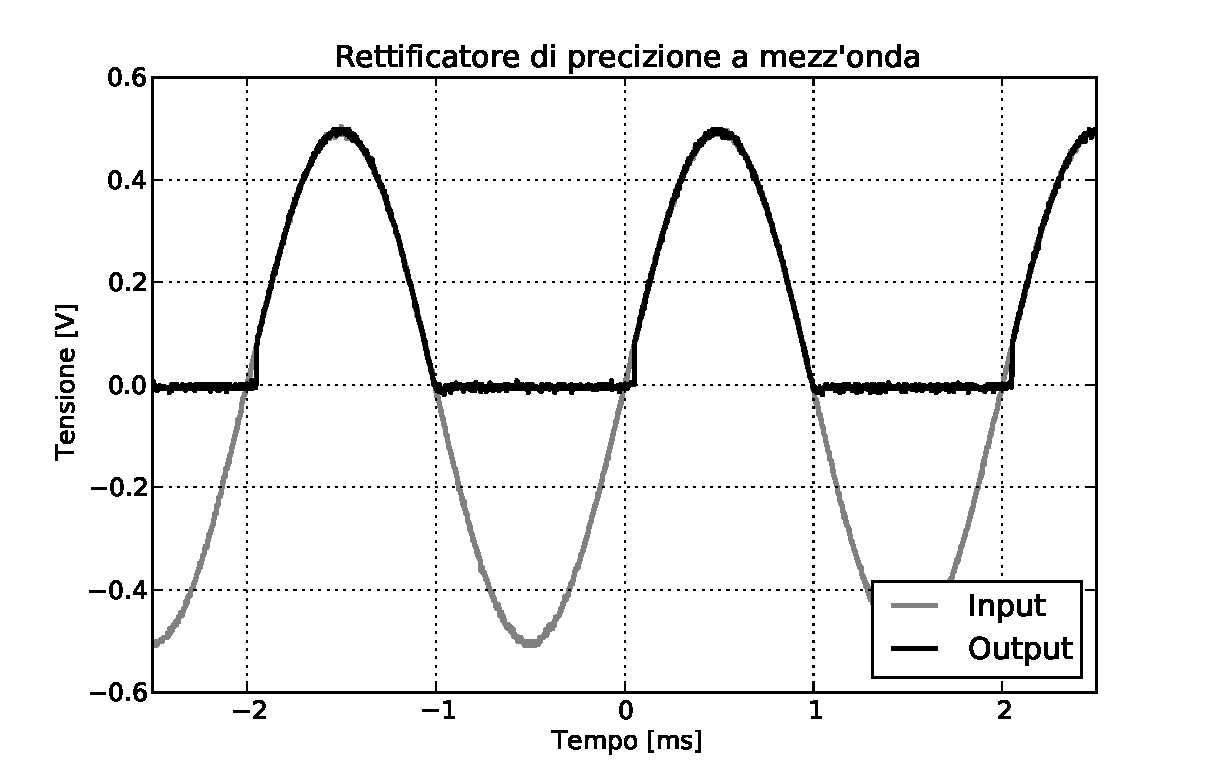
\includegraphics[height=0.32\textheight]{figure/rett.pdf}
    \caption{Input e output ($V_o$) del raddrizzatore a mezz'onda semplice (circuito \ref{fig:raddrizzatore5}).
        L'input è una sinusoide di 1 Vpp a 500 Hz.
        È visibile un certo ritardo del circuito a seguire l'andamento dell'ingresso, quando questa
        da negativo diventa positivo. Rispetto ad un raddrizzatore a diodi non è presente un offset di 0.6 V.}
    \label{fig:rett_graph5}
\end{SCfigure*}

\begin{SCfigure*}[][p]
    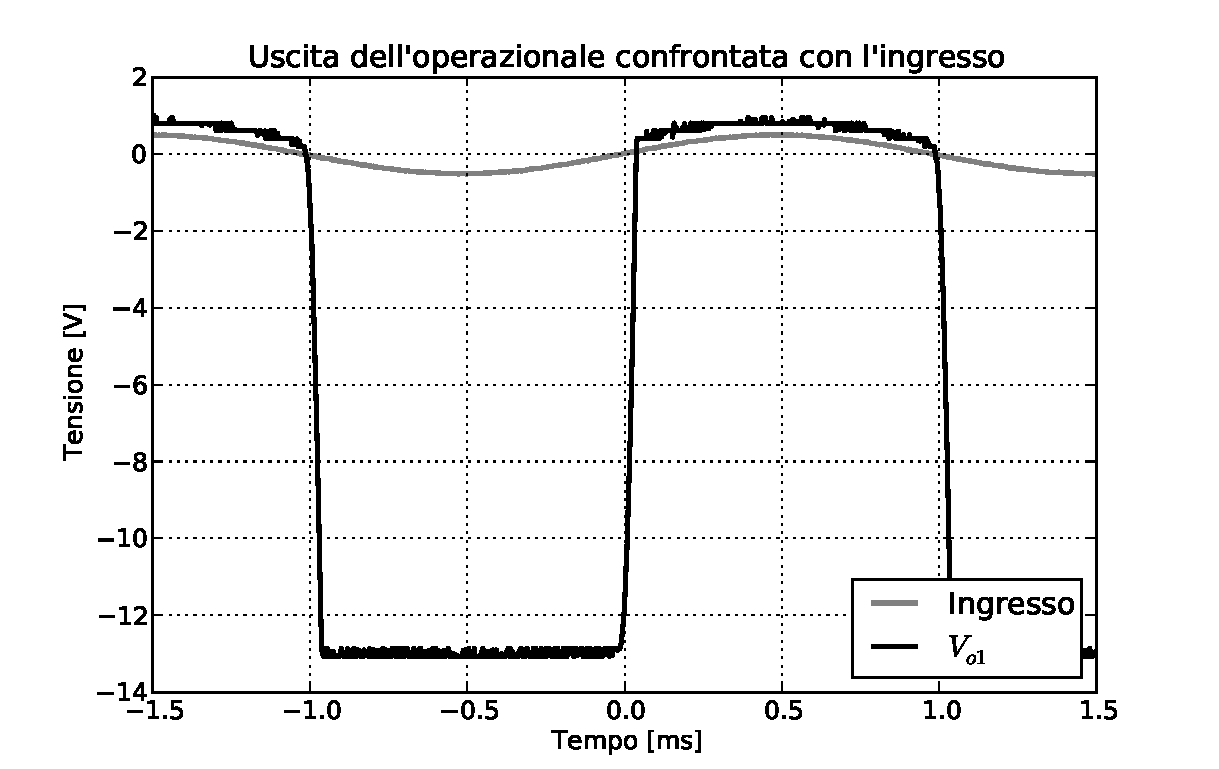
\includegraphics[height=0.32\textheight]{figure/rett_vo1.pdf}
    \caption{Input e tensione $V_{o1}$ all'uscita dell'amplificatore operazionale nel circuito \ref{fig:raddrizzatore5}.
        Si vede come l'operazionale vada in saturazione negativa (circa -13 V) e come impieghi un certo tempo a tornare in
        funzionamento lineare (per esempio al tempo t = 0). È inoltre visibile l'effetto della caduta in diretta del
        diodo, che ammonta a circa 0.4 V nel grafico. L'input è sempre una sinusoide 1 Vpp a 500 Hz.}
    \label{fig:rett_vo15}
\end{SCfigure*}

\begin{SCfigure*}[][p]
    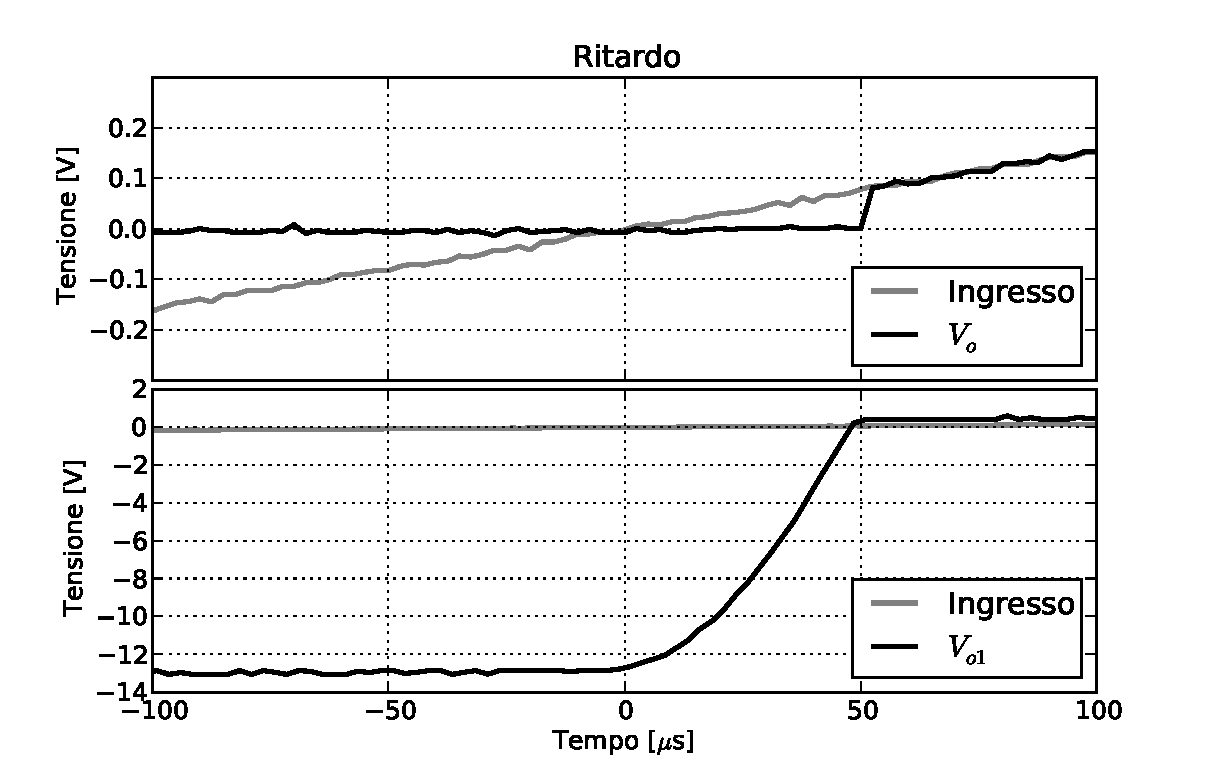
\includegraphics[height=0.32\textheight]{figure/rett_err.pdf}
    \caption{Questa immagine è un'ingrandimento delle precedenti due (figure \ref{fig:rett_graph5} e \ref{fig:rett_vo15})
        nella zona dove avviene il ritardo. Il ritardo è circa 50 $\mu$s, inspiegabile con il solo slew rate limitato
        dell'operazionale. Nel grafico in basso, la parte iniziale della curva nera (la parte meno pendente) è il momento
        in cui l'operazionale spende tempo ad uscire dalla saturazione.}
    \label{fig:rett_err5}
\end{SCfigure*}

Una soluzione elegante e semplice è quella di utilizzare un operazionale come indicato nel
circuito \ref{fig:raddrizzatore5}. Il circuito sfrutta la retroazione per far si che l'amplificatore
porti $V_o$ alla stessa tensione dell'ingresso, se quest'ultimo è positivo. Per fare ciò deve valere
$V\ped{o1} = V_o + V_d$, dove $V_d$ indica la caduta in diretta del diodo. Quando invece
l'ingresso è negativo l'opamp va in saturazione negativa e il diodo entra in interdizione.
In questa modalità l'amplificatore agisce in modalità open-loop.
$R\ped{L}$ gioca il ruolo di carico pilotato dal circuito.

Abbiamo quindi montato il circuito per verificarne il corretto funzionamento e i limiti operativi.
Abbiamo fornito in input delle onde sinusoidali di diverse frequenze (50 Hz, 500Hz, 5 kHz, 10 kHz)
e visualizzato l'output. Nelle figure \ref{fig:rett_graph5}, \ref{fig:rett_vo15} e \ref{fig:rett_err5}
sono mostrati tre grafici: nei primi due sono graficate 
le tensioni di input, $V_o$ e $V_{o1}$ e dimostra il funzionamento del circuito, il terzo è
semplicemente un ingrandimento della transizione da $V_o = 0$ V a $V_o = V\ped{in}$.
L'operazionale impiega un certo tempo, variabile
con la frequenza del segnale, per uscire dallo stato di saturazione negativa e raggiungere la zona di
funzionamento lineare. La transizione opposta, da uscita uguale al segnale a $V_o = 0$ V, non presenta
questo tipo di imprecisione.

Come mai c'è un ritardo? 
La tensione di offset in questo caso è troppo piccola per avere effetti cospicui come quelli osservati.
Inizialmente abbiamo pensato che il ritardo nella risposta fosse dovuto allo slew rate,
ovvero al fatto che per passare da - 15 V a circa 0 V l'operazionale UA741 ha bisogno di circa
30 $\mu$s (assumendo uno slew rate di 0.5 V/$\mu$s, misurato nelle precedenti relazioni).
Tuttavia abbiamo osservato ritardi variabili fino a 160 $\mu$s per cui, anche se lo slew rate
di sicuro gioca un ruolo, deve esserci qualcos'altro a ritardare ulteriormente l'amplificatore.
Questo ``qualcos'altro'' è il fatto che, per uscire dall'interdizione o dalla saturazione, i transistor
che compongono l'operazionale
impiegano un certo tempo. Questo tempo è tanto minore quanto maggiore è la derivata della
tensione, poiché questo causa cambiamenti più repentini e correnti più alte all'interno dell'operazionale.

Questo spiega il comportamento del circuito e anche la diminuzione del tempo di commutazione all'aumentare
della frequenza. Spiega inoltre perché questo ritardo avvenga solo con una tensione in ingresso crescente ma
non quando decresce.

\paragraph{Rettificatore a mezz'onda migliorato.}

Poiché stiamo tentando di costruire un raddrizzatore a mezz'onda di precisione, vogliamo eliminare
il problema presentato nel paragrafo precedente. Vogliamo quindi impedire che l'operazionale vada
in saturazione negativa per evitare i problemi connessi alla commutazione. Ancora meglio, vorremmo
tenere il suo output vicino al riferimento, in modo da ridurre possibili problemi di slew rate.

Abbiamo quindi realizzato il circuito \ref{fig:rad_ott5}. In questo caso il raddrizzatore è invertente,
cioè mantiene solo le parti dell'input negative, rendendole però positive.

Riassumiamo il funzionamento del circuito:

\begin{itemize}
    \item{Se $V\ped{in} > 0$: il diodo $D_2$ è interdetto e il circuito funziona come un amplificatore
        invertente, con guadagno 1 se $R_1 = R_2$. $D_1$ fa in modo che $V\ped{o1} = V_o + V_d$.}
    \item{Se $V\ped{in} < 0$: l'operazionale tenta di andare in saturazione negativa, per cui $D_1$ è
        interdetto e la retroazione non funziona più. Poiché l'ingresso invertente è un ground virtuale
        e il carico è a comune si ha $V_o = 0$ V. Il diodo $D_2$ impedisce all'operazionale di andare in saturazione
        negativa e mantiene la sua uscita a $-V_d$.}
\end{itemize}

Abbiamo quindi analizzato il comportamento del circuito per la stessa onda sinusoidale 1 Vpp e per le stesse
frequenze del circuito precedente. In figura \ref{fig:radd_ott_graph5} è mostrato il grafico con le misure di
$V_o$ e $V_{o1}$ e dell'ingresso alla frequenza di 500 Hz. In questo caso abbiamo rilevato un comportamento
molto più pulito, con commutazioni con ritardi molto meno marcati (generalmente da 3 a 5 microsecondi).
Inoltre, si osserve la figura riferita sopra, $V_{o1}$ non è mai sceso oltre i - 0.5 V.

\begin{SCfigure*}
    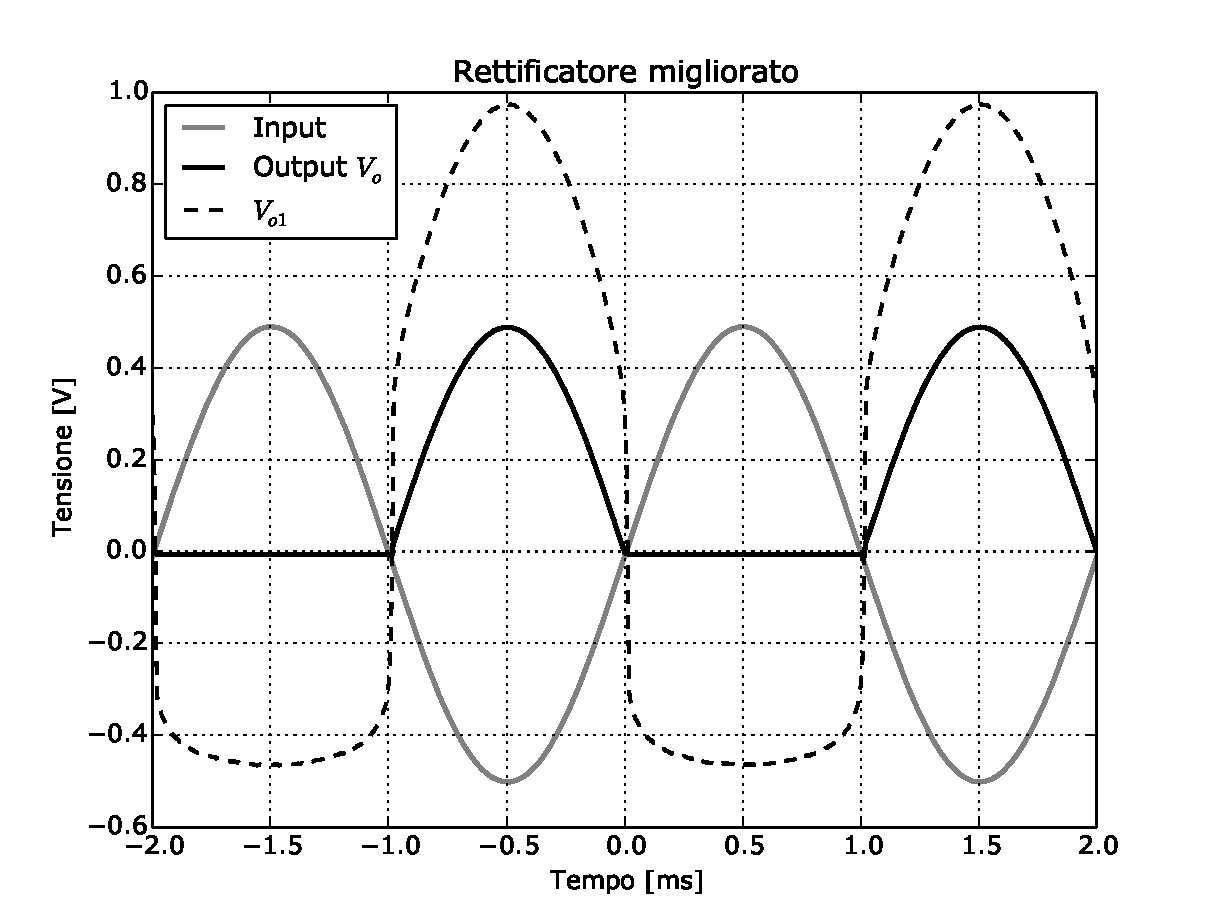
\includegraphics[width=1.5\columnwidth]{figure/radd_ott_graph.pdf}
    \caption{Il raddrizzatore ottimizzato produce un output molto più pulito (senza ritardi) mantenendo $V_{o1}$ vicino a 0 V.
	Il raddrizzatore in questo caso mantiene le semionde negative raddrizzandole. $V_{o1}$ è circa 0.5 V più alta di $V_o$,
	come ci si aspetta dalla caduta in polarizzazione diretta del diodo. Il fatto che la curva tratteggiata sia tonda in basso è
	dovuto alla caratteristica del diodo.}
    \label{fig:radd_ott_graph5}
\end{SCfigure*}

\paragraph{Amplificatore differenziale.}

Nella fase successiva dell'esperienza, abbiamo studiato gli amplificatori strumentali, ovvero degli
amplificatore differenziali che sono utili per eliminare il rumore nel caso in cui si debbano fare misure
utilizzando cavi lunghi (per esempio un apparato sperimentale e apparecchi di misura dall'altro lato
del laboratorio o in locali adiacenti). La lunghezza dei cavi introduce problematiche legate al rumore che non
sorgono nel caso cavi corti. Per esempio, in un caso del genere può essere conveniente collegare usare la terra
come comune, cosa che però induce disturbi a causa del fatto che i punti in cui l'impianto elettrico è messo a terra
possono trovarsi a potenziali diversi. Inoltre sono più forti i disturbi generati da onde radio, onde elettromagnetiche
generate dalla rete e da altra strumentazione

Per evitare i problemi dovuti al rumore si più utilizzare un amplificatore differenziale in un circuito come il
\ref{fig:diff5}. Nel circuito $V\ped{in}$ rappresenta il segnale da misurare (nel nostro caso una tensione DC).
In questo caso abbiamo usato un amplificatore differenziale costruito con un UA741, che è costituito dall'operazionale
e da tutte le resistenze visibili nel circuito. Il trimmer serve per regolare con precisione le resistenze,
poiché è impossibile trovare delle resistenze tutte uguali. Per eseguire la taratura abbiamo collegato i due ingressi
($V\ped{in} = 0$) e abbiamo modificato la resistenza fino a che l'output non è diventato nullo. 
Per simulare la presenza di rumore, abbiamo utilizzato il generatore di forme d'onda collegato tra il segnale e comune.
Le resistenze sono state scelte per amplificare l'ingresso differenziale di un fattore 2.

Lo scopo del circuito è quello di amplificare solo il segnale con l'amplificatore differenziale, mentre il rumore,
essendo presente in entrambi gli input viene scartato.

Il test del funzionamento è semplice: si visualizza l'output e il rumore (il segnale generato dal generatore di funzioni)
e variando frequenza, ampiezza e forma del rumore si verifica che il segnale amplificato non venga modificato.
Abbiamo quindi posto $V\ped{in} = 1$ v e provato con sinusoidi, onde quadre, triangoli, rampe e altre funzioni a frequenze
da 50 Hz a 100 kHz. Il circuito si è comportato bene, anche se quando il rumore ha un'ampiezza grande (per esempio 10 Vpp)
si nota che l'output, invece di essere piatto, è una onda sinusoidale di circa 5 mVpp. In ogni caso un rumore di tale
ampiezza in pratica non si ha mai. L'intero problema del rumore si ha solo se si vuole misurare un segnale comparabile
con la dimensione del rumore, cioè di qualche millivolt.

\paragraph{Instrumental amplifier AD622.}

\begin{figure*}[t]
    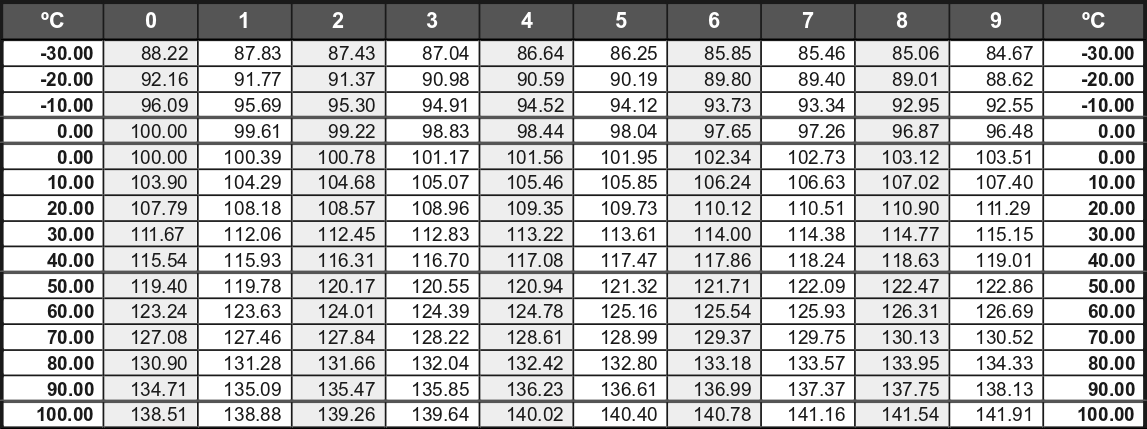
\includegraphics[width=\textwidth]{figure/temp.png}
    \caption{Valori della resistenza PT100 per varie temperature.}
    \label{fig:temp5}
\end{figure*}

L'amplificatore differenziale studiato nel paragrafo precedente non è privo di problemi, prima di tutto la piccola impedenza
in ingresso. Inoltre spesso è comodo poter variare il guadagno senza dover cambiare le resistenze e ricalibrare il circuito.
Per risolvere questo problema è possibile usare un circuito costruito con 3 amplificatori operazionali; un tale circuito sfrutta
l'elevata impedenza degli ingressi degli opamp e non sarebbe complicato da costruire. Tuttavia è ancora più comodo e preciso
utilizzare un integrato che contiene al suo interno l'intero circuito. In questo modo si ha anche il beneficio aggiuntivo di avere
delle resistenze costruite in modo tale da non sbilanciare il circuito. Questi integrati sono anche chiamati instrumental amplifiers.

L'integrato da noi utilizzato è l'AD622, che viene venduto in un package simile a quello di un operazionale,
con la particolarità che va connesso a comune e che ha due piedini che devono essere collegati ad una resistenza
variabile. Cambiando valore della resistenza è possibile variare il guadagno del circuito.

Per prendere confidenza con l'AD622 abbiamo realizzato il circuito \ref{fig:inst_amp5}. Il circuito non fa altro che
amplificare lo sbilanciamento di un ponte di Wheatstone. La resistenza $R_s$ è stata montata fisicamente lontana
dalle altre per poter essere riscaldata e raffreddata senza interferire con le altre.

Abbiamo quindi visualizzato l'output del circuito. In condizioni di operazione a temperatura ambiente l'output valeva
$- 1040 \pm 10$ mV a causa del sempre presente sbilanciamento delle resistenze. Il guadagno è stato scelto in modo 
 da avere un output in queste condizioni di circa 1 V. Successivamente abbiamo riscaldato la resistenza $R_s$
con un dito. In queste condizioni operative abbiamo misurato $- 1210 \pm 10$ mV in uscita. Raffreddando invece la resistenza
con una bomboletta di refrigerante abbiamo registrato $-460 \pm 10$ mV. Poiché il valore a temperatura ambiente
è negativo abbiamo che $R_s$ è leggermente più piccola dell'altra resistenza da 100 \si{\ohm} (il ponte di Wheatstone
può essere visto come due partitori e l'output del partitore con $R_s$ deve essere più piccolo dell'altro).
All'aumentare della temperatura il valore di resistenza diminuisce, poiché
l'uscita scende, quindi il coefficiente di temperatura è negativo.

%Le specifiche delle resistenze indicano che il coefficiente di temperatura è di circa -20 \si{\milli\ohm\per\celsius},
%per cui possiamo stimare in maniera molto rozza la temperatura nei due casi riportati sopra. La stima collo spray freddo può
%essere completamente sbagliata, poiché la dipendenza dalla temperatura in realtà è non lineare e il coefficiente
%diventa positivo sotto di una certa temperatura.

%Assumendo un guadagno A di circa 300 dell'INA (INstrumental Amplifier), si può calcolare la variazione di tensione ai capi di
%$R_s$ ($\Delta V\ped{R_s}$) e quindi calcolare la variazione di $R_s$ utilizzando la formula per il partitore di tensione

%\begin{equation}
%    \Delta V\ped{R_s} = \frac{\Delta V\ped{out}}{A} \implies \Delta R_s = \frac{1001 * \Delta V\ped{R_s}}{V_w}
%\end{equation}
% 
%dove $V_w = 5$ V indica l'alimentazione del ponte di Wheatstone e 1001 è il rapporto (approssimato) tra la somma delle
%resistenze del partitore e $R_s$.

%Possiamo fare anche una veloce stima del coefficiente di temperatura della resistenza supponendo che la temperatura
%corporea fosse 37$^\circ$ C e che la bomboletta abbassasse la temperatura a circa -20$^\circ$ C (questo lo verificheremo
%nel prossimo paragrafo). La tensione all'ingresso non invertente vale
%
%\begin{equation}
%    V^+ = V_w * \frac{R_s}{R_s + R}
%\end{equation}
%%
%dove $V_w = 5$ V e R = \SI{100}{\kilo\ohm}. Una formula simile vale per l'ingresso invertente, ma con $R_s$ sostituito con
%r = 100 \si{\ohm}. L'uscita dall'amplificatore strumentale è
%
%\begin{equation}
%    V\ped{out} = \frac{AV_w}{R}\left(R_s - r\right)
%\end{equation}
%%
%in questa formula A è il guadagno (non misurato) dell'amplificatore, inoltre abbiamo considerato le due resistenze da 100k
%identiche e r e $R_s$ sono state trascurate a denominatore. Ricavando $R_s$:
%
%\begin{equation}
%    R_s = \frac{V\ped{out}R}{AV_w} - r
%\end{equation}
%%
%da cui
%\begin{equation}
%   \Delta R_s = \frac{\Delta V\ped{out}R}{AV_w}
%\end{equation}
%
%Il coefficiente di temperatura è dato da
%
%\begin{equation}
%    \alpha = \frac{\Delta R_s}{\Delta T} = \frac{\Delta V\ped{out}R}{AV_wT} = 
%\end{equation}

\paragraph{Misura di temperatura.}

\begin{figure}
    \centering
    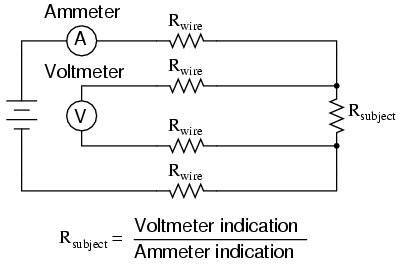
\includegraphics[width=0.9\columnwidth]{figure/scopiazzo.png}
    \caption{Misura a 4 cavi.}
    \label{fig:scopiazzo5}
\end{figure}

Come ultima misura della giornata, abbiamo usato una resistenza al platino PT100 per la misura di temperatura con il multimetro,
in misurazione con 4 cavi. La resistenza al platino che ci è stata fornita ha una resistenza di 100 \si{\ohm} alla temperatura
di 0 $^\circ$C. Le resistenze al platino hanno delle variazioni ben precise di resistenza al variare della temperatura e hanno
tolleranze piccole. Si trovano tabulati i valori di resistenza per ogni grado centigrado (figura \ref{fig:temp5}),
in modo da poter fare facilmente la conversione tra resistenza e temperatura.

Per questo tipo di misura è importante riuscire a misurare esattamente la resistenza, senza introdurre errori sistematici
dovuti all'impedenza dei cavi di collegamento. Poiché la resistenza è da soli 100 \si{\ohm} anche una cavo con un impedenza piuttosto
piccola, per esempio 1 \si{\ohm} (che potrebbe essere la resistenza di un cavo sottile abbastanza lungo), ci fa compiere un errore
dell'1\%, cioè di circa 3 $^\circ$C. Per ovviare a questo inconveniente si utilizza la misura a 4 fili. In questa modalità di misura
(figura \ref{fig:scopiazzo5}),
invece di utilizzare due fili, far scorrere la corrente in un circolo e misurare la caduta di potenziale (che include la caduta dovuta
ai cavi di collegamento), se ne utilizzano 4: 2 formano un loop in cui è imposta una corrente dall'esterno, gli altri due servono
alla misura della tensione. Su un anello si misura la corrente, che passa sicuramente attraverso la reistenza in esame $R\ped{subject}$,
nell'altro si misura la tensione ai capi, utilizzando un voltmetro che fa passare pochissima corrente.
Utilizzando la legge di Ohm si ottiene una misura molto più precisa, poiché
nel ramo di misura della tensione la corrente è piccolissima. Può sembrare che questa modalità di misura non faccia quadagnare nulla,
tuttavia il trucco stà nel fatto che la corrente che passa attraverso un amperometro è alta, mentre quella in un voltmetro è bassa.
Combinando i due strumenti si ha che la misura di tensione è influenzata praticamente solo dalla $R\ped{subject}$ poiché attraverso di
essa passa molta corrente, mentre nelle resistenze dei cavi di collegamento del voltmetro ne passa pochissima.

Abbiamo quindi simulato la resistenza dei cavi con delle resistenze da 10 \si{\ohm}. A temperatura ambiente abbiamo misurato
112.00 \si{\ohm} che indica una temperatura di 31 $^\circ$C (in lab fa un gran caldo!). Con la misura a due fili si otteneva 
invece 134 \si{\ohm} (circa $112 + 2 \times 10$), che significherebbe 78 $^\circ$C. Anche se questo è un esempio artificioso,
si capisce ben che bastano pochi Ohm sui cavi di collegamento per rendere completamente inutile la misura. Riscaldando la resistenza con le dita abbiamo
invece letto 114.32 \si{\ohm} (37 $^\circ$C), mentre raffreddandola con lo spray abbiamo misurato 89,5 \si{\ohm} (-27 $^\circ$C).
